\chapter{Types of Learning}
\lecture{3}{16 Sep.}{}

\begin{prev}
    \autoref{sec:pla} produced one complete learning model: PLA takes a linearly
    separable \(\mathcal{D}\) and the perceptrons \(\mathcal{H}\), and returns a
    hypothesis \(g\). That is one point in a very large space of possibilities.
\end{prev}

The frame of \autoref{sec:components} has several slots --- the output space
\(\mathcal{Y}\), the labels \(y_n\), the way the data reaches us, the input space
\(\mathcal{X}\) --- and so far every one of them has been filled in the simplest
way available. This chapter varies them one at a time, which is the cheapest way
to see what the frame can hold. Nothing here is proved; the point is a map of
the territory, and the names on it recur for the rest of the course.

\section{Learning with Different Output Space
\texorpdfstring{\(\mathcal{Y}\)}{Y}}\label{sec:outspace}

\source{slides p.2--8}

\subsection{The Credit Approval Problem Revisited}

Credit approval answers one yes/no question, so its output space has exactly two
elements.

\begin{center}
    \begin{adjustbox}{max width=\textwidth}
        \begin{tikzpicture}
            \node[mlbox, minimum width=4.2cm] (f) at (0,2.25)
                {unknown target function\\
                 \(f\colon \mathcal{X} \to\) \textcolor{WildStrawberry}{\(\bm{\mathcal{Y}}\)}\\[2pt]
                 {\scriptsize (ideal target formula)}};
            \node[mlbox, minimum width=5.2cm] (D) at (0,0)
                {training examples\\
                 \(\mathcal{D}\colon (\bm{x}_1, y_1), \dots , (\bm{x}_N, y_N)\)\\[2pt]
                 {\scriptsize (historical records)}};
            \node[mlop, minimum width=2.4cm] (A) at (5.4,0)
                {learning\\algorithm\\\(\mathcal{A}\)};
            \node[mlbox, minimum width=4.4cm] (g) at (10.2,0)
                {final hypothesis\\\(g \approx f\)\\[2pt]
                 {\scriptsize (`learned' formula to be used)}};
            \node[mlbox, minimum width=3.4cm] (H) at (5.4,-2.25)
                {hypothesis set\\\(\mathcal{H}\)\\[2pt]
                 {\scriptsize (set of candidate formulas)}};
            \draw[mlarrow] (f) -- (D);
            \draw[mlarrow] (D) -- (A);
            \draw[mlarrow] (A) -- (g);
            \draw[mlarrow] (H) -- (A);
            \node[mlbox, minimum width=4.8cm] (side) at (8.30,2.55)
                {\scriptsize\textbf{Applicant Information}\\[3pt] \scriptsize\begin{tabular}{@{}lr@{}}age & 23 years\\ gender & female\\ annual salary & NTD 1,000,000\\year in residence & 1 year\\ year in job & 0.5 year\\current debt & 200,000\\\midrule credit? & \textcolor{WildStrawberry}{\(\left\{ -1, +1 \right\}\)}\\\end{tabular}};
        \end{tikzpicture}
    \end{adjustbox}
\end{center}

\begin{moral}
    \(\mathcal{Y} = \left\{ -1, +1 \right\}\): binary classification.
\end{moral}

\subsection{Binary Classification}

\begin{definition}[Binary classification]\label{def:binary}
    A learning problem whose output space has exactly two elements,
    \(\mathcal{Y} = \left\{ -1, +1 \right\}\), is called \vocab{binary
    classification}. The two elements are only names: good/bad, spam/non-spam,
    sick/not sick.
\end{definition}

The same output space covers an enormous range of questions:

\begin{itemize}
    \item credit approve/disapprove;
    \item email spam/non-spam;
    \item patient sick/not sick;
    \item ad profitable/not profitable;
    \item answer correct/incorrect (KDDCup 2010).
\end{itemize}

Geometrically it is the picture we already know --- a boundary with one class on
each side, easy or hard depending on how the data falls.

\begin{center}
    \begin{adjustbox}{max width=\textwidth}
        \begin{tikzpicture}
            \begin{scope}
                \fill[neghalf] (0,0) -- (1.5,0) -- (1.8,3.2) -- (0,3.2) -- cycle;
                \fill[poshalf] (1.5,0) -- (3.2,0) -- (3.2,3.2) -- (1.8,3.2) -- cycle;
                \draw[sepline] (1.5,0) -- (1.8,3.2);
                \draw[black!45] (0,0) rectangle (3.2,3.2);
                \foreach \p in {(0.5,2.6), (0.9,1.6), (0.4,0.8), (1.2,2.9),
                    (0.7,2.0)}{\node[dneg] at \p {\(\times\)};}
                \foreach \p in {(2.3,2.6), (2.7,1.5), (2.0,0.9), (2.9,2.3),
                    (2.4,1.9)}{\node[dpos] at \p {};}
            \end{scope}
            \begin{scope}[xshift=4.0cm]
                \fill[poshalf] (0,3.2) -- (3.2,0) -- (3.2,3.2) -- cycle;
                \fill[neghalf] (0,3.2) -- (3.2,0) -- (0,0) -- cycle;
                \draw[sepline] (0,3.2) -- (3.2,0);
                \draw[black!45] (0,0) rectangle (3.2,3.2);
                \foreach \p in {(1.5,2.4), (2.2,2.8), (2.6,1.6), (1.9,1.9),
                    (2.9,2.4)}{\node[dpos] at \p {};}
                \foreach \p in {(0.5,0.9), (1.2,1.0), (0.8,1.9), (1.8,0.6),
                    (0.4,2.0)}{\node[dneg] at \p {\(\times\)};}
                \node[dneg] at (2.4,2.1) {\(\times\)};
                \node[dpos] at (0.9,0.7) {};
            \end{scope}
            \begin{scope}[xshift=8.0cm]
                \fill[neghalf] (0,0) rectangle (3.2,3.2);
                \fill[poshalf] (1.6,1.6) circle (1.0);
                \draw[sepline] (1.6,1.6) circle (1.0);
                \draw[black!45] (0,0) rectangle (3.2,3.2);
                \foreach \p in {(1.6,1.6), (1.2,1.9), (2.0,1.3), (1.5,1.1),
                    (2.1,1.9)}{\node[dpos] at \p {};}
                \foreach \p in {(0.4,0.5), (2.9,0.6), (0.5,2.9), (2.9,2.8),
                    (1.6,3.0), (0.3,1.6)}{\node[dneg] at \p {\(\times\)};}
            \end{scope}
        \end{tikzpicture}
    \end{adjustbox}
\end{center}

\begin{moral}
    A core and important problem, with many tools that serve as building blocks
    of other tools.
\end{moral}

\subsection{Multiclass Classification}

\begin{definition}[Multiclass classification]\label{def:multiclass}
    A learning problem whose output space is finite and explicitly listed,
    \(\mathcal{Y} = \left\{ 1, 2, \dots , K \right\}\) with \(K \ge 2\), is
    called \vocab{multiclass classification}; \autoref{def:binary} is the
    special case \(K = 2\).
\end{definition}

\begin{eg}[Coin recognition]\label{eg:coins}
    Classify US coins --- \(1\)c, \(5\)c, \(10\)c, \(25\)c --- by their
    \((\text{size}, \text{mass})\). The four denominations form four clusters,
    because a heavier coin is usually a larger one.
    \begin{center}
        \begin{tikzpicture}
                \draw[plotbox] (0,0) rectangle (3.20,3.20);
                \node[font=\tiny, below] at (1.60,-0.02) {Size};
                \node[font=\tiny, rotate=90, above] at (-0.02,1.60) {Mass};
                \node[dcls=Goldenrod] at (0.663,0.594) {};
                \node[dcls=Goldenrod] at (0.668,0.462) {};
                \node[dcls=Goldenrod] at (0.555,0.478) {};
                \node[dcls=Goldenrod] at (0.882,0.580) {};
                \node[dcls=Goldenrod] at (0.870,0.552) {};
                \node[dcls=Goldenrod] at (0.767,0.542) {};
                \node[dcls=Goldenrod] at (0.437,0.649) {};
                \node[dcls=Goldenrod] at (0.785,0.592) {};
                \node[dcls=Goldenrod] at (0.433,0.233) {};
                \node[dcls=Goldenrod] at (0.562,0.437) {};
                \node[dcls=Goldenrod] at (0.753,0.505) {};
                \node[dcls=Goldenrod] at (0.787,0.409) {};
                \node[dcls=Goldenrod] at (0.753,0.575) {};
                \node[dcls=Goldenrod] at (0.598,0.787) {};
                \node[font=\tiny, Goldenrod!60!black] at (0.320,0.800) {\(10\)};
                \node[dcls=RoyalBlue] at (1.241,1.248) {};
                \node[dcls=RoyalBlue] at (1.053,0.938) {};
                \node[dcls=RoyalBlue] at (1.097,1.039) {};
                \node[dcls=RoyalBlue] at (1.253,1.096) {};
                \node[dcls=RoyalBlue] at (1.080,0.903) {};
                \node[dcls=RoyalBlue] at (1.069,1.251) {};
                \node[dcls=RoyalBlue] at (1.023,1.095) {};
                \node[dcls=RoyalBlue] at (1.220,0.818) {};
                \node[dcls=RoyalBlue] at (1.160,1.265) {};
                \node[dcls=RoyalBlue] at (0.830,1.005) {};
                \node[dcls=RoyalBlue] at (1.135,0.925) {};
                \node[dcls=RoyalBlue] at (1.232,1.046) {};
                \node[dcls=RoyalBlue] at (0.918,1.188) {};
                \node[dcls=RoyalBlue] at (1.259,1.207) {};
                \node[font=\tiny, RoyalBlue!60!black] at (0.768,1.344) {\(1\)};
                \node[dcls=RedOrange] at (1.918,1.696) {};
                \node[dcls=RedOrange] at (1.685,1.403) {};
                \node[dcls=RedOrange] at (1.772,1.524) {};
                \node[dcls=RedOrange] at (1.584,1.409) {};
                \node[dcls=RedOrange] at (1.494,1.539) {};
                \node[dcls=RedOrange] at (1.891,1.274) {};
                \node[dcls=RedOrange] at (1.407,1.674) {};
                \node[dcls=RedOrange] at (1.918,1.734) {};
                \node[dcls=RedOrange] at (1.330,1.189) {};
                \node[dcls=RedOrange] at (1.727,1.502) {};
                \node[dcls=RedOrange] at (1.467,1.804) {};
                \node[dcls=RedOrange] at (1.858,1.660) {};
                \node[dcls=RedOrange] at (1.707,1.708) {};
                \node[dcls=RedOrange] at (1.945,1.741) {};
                \node[font=\tiny, RedOrange!60!black] at (1.280,1.920) {\(5\)};
                \node[dcls=ForestGreen] at (2.468,2.633) {};
                \node[dcls=ForestGreen] at (2.067,2.774) {};
                \node[dcls=ForestGreen] at (2.551,2.630) {};
                \node[dcls=ForestGreen] at (1.989,2.406) {};
                \node[dcls=ForestGreen] at (2.530,2.180) {};
                \node[dcls=ForestGreen] at (2.333,2.724) {};
                \node[dcls=ForestGreen] at (2.116,2.837) {};
                \node[dcls=ForestGreen] at (2.474,2.499) {};
                \node[dcls=ForestGreen] at (2.430,2.653) {};
                \node[dcls=ForestGreen] at (2.391,2.748) {};
                \node[dcls=ForestGreen] at (2.241,2.448) {};
                \node[dcls=ForestGreen] at (2.568,2.533) {};
                \node[dcls=ForestGreen] at (2.199,2.710) {};
                \node[dcls=ForestGreen] at (2.649,2.443) {};
                \node[font=\tiny, ForestGreen!60!black] at (1.984,2.816) {\(25\)};
        \end{tikzpicture}
    \end{center}
    Here \(\mathcal{Y} = \left\{ 1\text{c}, 5\text{c}, 10\text{c}, 25\text{c}
    \right\}\), so \(K = 4\).
\end{eg}

Other multiclass problems: written digits \(\Rightarrow 0, 1, \dots , 9\);
pictures \(\Rightarrow\) apple, orange, strawberry; emails \(\Rightarrow\) spam,
primary, social, promotion, update (Google).

\begin{moral}
    Many applications in practice, especially for `recognition'.
\end{moral}

\subsection{Regression}

\begin{definition}[Regression]\label{def:regression}
    A learning problem whose output space is the whole real line,
    \(\mathcal{Y} = \mathbb{R}\), is called \vocab{regression}; if the output is
    confined to an interval, \(\mathcal{Y} = [\text{lower}, \text{upper}]
    \subset \mathbb{R}\), it is \vocab{bounded regression}. The difference from
    classification is that \(\mathcal{Y}\) now carries an order and a distance,
    so being wrong by a little is better than being wrong by a lot.
\end{definition}

Keep the patient, change the question, and the output space changes with it:

\begin{itemize}
    \item binary classification: patient features \(\Rightarrow\) sick or not;
    \item multiclass classification: patient features \(\Rightarrow\) which type
        of cancer;
    \item \emph{regression}: patient features \(\Rightarrow\) how many days
        before recovery.
\end{itemize}

Regression was studied deeply in statistics long before machine learning
existed, which is why so many of its tools arrive ready-made. Other regression
problems: company data \(\Rightarrow\) stock price; climate data
\(\Rightarrow\) temperature.

\begin{moral}
    Also core and important, with many `statistical' tools as building blocks of
    other tools.
\end{moral}

\subsection{Structured Learning}

\begin{definition}[Structured learning]\label{def:structured}
    \vocab{Structured learning} is a learning problem whose outputs are
    composite objects --- a tag for every word of a sentence, a folding of a
    protein, a parse tree --- whose parts constrain one another. Formally
    \(\mathcal{Y}\) is still a finite set of `classes', but an enormous one that
    is defined implicitly by those constraints rather than enumerated.
\end{definition}

\begin{eg}[Sequence tagging]
    Multiclass classification sends a word to a word class. Structured
    learning sends a whole sentence to a structure --- the class of every word
    at once:
    \[
        \underbrace{\text{I}}_{\text{pronoun}} \;
        \underbrace{\text{love}}_{\text{verb}} \;
        \underbrace{\text{ML}}_{\text{noun}}
    \]
    so that \(\mathcal{Y} = \left\{ \mathrm{PVN}, \mathrm{PVP}, \mathrm{NVN},
    \mathrm{PV}, \dots \right\}\), not including \(\mathrm{VVVVV}\).
\end{eg}

That exclusion is the whole difficulty. The output space is a huge multiclass
problem --- a structure is a kind of hyperclass --- but without an
\emph{explicit} class definition: the valid structures are constrained by
grammar, and nobody wrote the list down. Other structured problems: protein data
\(\Rightarrow\) protein folding; speech data \(\Rightarrow\) speech parse tree.

\begin{moral}
    A fancy but complicated learning problem.
\end{moral}

\subsection{Mini Summary}

\begin{note}[Learning with different output space \(\mathcal{Y}\)]
    \hfill
    \begin{itemize}
        \item binary classification: \(\mathcal{Y} = \left\{ -1, +1 \right\}\);
        \item multiclass classification:
            \(\mathcal{Y} = \left\{ 1, 2, \dots , K \right\}\);
        \item regression: \(\mathcal{Y} = \mathbb{R}\);
        \item structured learning: \(\mathcal{Y} = \text{structures}\);
        \item \ldots{} and a lot more!!
    \end{itemize}
\end{note}

\begin{moral}
    Core tools: binary classification and regression.
\end{moral}

\begin{exercise}[Fun Time]
    The entrance system of the school gym, which does automatic face recognition
    based on machine learning, is built to charge four different groups of users
    differently: Staff, Student, Professor, Other. What type of learning problem
    best fits the need of the system?
    \begin{enumerate}[(1)]
        \item binary classification;
        \item multiclass classification;
        \item regression;
        \item structured learning.
    \end{enumerate}
\end{exercise}

\begin{proof}[Reference Answer]
    (2). There is an `explicit' \(\mathcal{Y}\) that contains four classes.
\end{proof}

\section{Learning with Different Data Label
\texorpdfstring{\(y_n\)}{yn}}\label{sec:labels}

\source{slides p.9--15}

\subsection{Supervised Learning}

\begin{definition}[Supervised learning]\label{def:supervised}
    Learning from data in which every input carries its own label,
    \[
        \mathcal{D} = \left\{ (\bm{x}_n, y_n) \right\}_{n=1}^{N} ,
    \]
    is called \vocab{supervised learning}. This is the only kind we have used so
    far.
\end{definition}

Everything so far has quietly assumed that the data arrives fully labelled.

\begin{center}
    \begin{adjustbox}{max width=\textwidth}
        \begin{tikzpicture}
            \node[mlbox, minimum width=4.2cm] (f) at (0,2.25)
                {unknown target function\\
                 \(f\colon \mathcal{X} \to \mathcal{Y}\)\\[2pt]
                 {\scriptsize (ideal target formula)}};
            \node[mlbox, minimum width=5.2cm, draw=WildStrawberry, very thick] (D) at (0,0)
                {training examples\\
                 \(\mathcal{D}\colon (\bm{x}_1, y_1), \dots , (\bm{x}_N, y_N)\)\\[2pt]
                 {\scriptsize (historical records)}};
            \node[mlop, minimum width=2.4cm] (A) at (5.4,0)
                {learning\\algorithm\\\(\mathcal{A}\)};
            \node[mlbox, minimum width=4.4cm] (g) at (10.2,0)
                {final hypothesis\\\(g \approx f\)\\[2pt]
                 {\scriptsize (`learned' formula to be used)}};
            \node[mlbox, minimum width=3.4cm] (H) at (5.4,-2.25)
                {hypothesis set\\\(\mathcal{H}\)\\[2pt]
                 {\scriptsize (set of candidate formulas)}};
            \draw[mlarrow] (f) -- (D);
            \draw[mlarrow] (D) -- (A);
            \draw[mlarrow] (A) -- (g);
            \draw[mlarrow] (H) -- (A);
        \end{tikzpicture}
    \end{adjustbox}
\end{center}

\begin{moral}
    Supervised learning: every \(\bm{x}_n\) comes with a corresponding
    \(y_n\).
\end{moral}

\subsection{Unsupervised Learning}

\begin{definition}[Unsupervised learning]\label{def:unsupervised}
    Learning from data that carries no labels at all,
    \[
        \mathcal{D} = \left\{ \bm{x}_n \right\}_{n=1}^{N} ,
    \]
    is called \vocab{unsupervised learning}. With no \(y_n\) there is no target
    \(f\) to approximate in the sense of \autoref{sec:components}, so what
    counts as a good \(g\) has to be decided separately for each problem.
\end{definition}

Now delete the labels. The coins are still there, and they still fall into
clusters --- but nothing says which cluster is the quarter.

\begin{center}
    \begin{adjustbox}{max width=\textwidth}
        \begin{tikzpicture}
            \begin{scope}
                \draw[plotbox] (0,0) rectangle (3.20,3.20);
                \node[font=\tiny, below] at (1.60,-0.02) {Size};
                \node[font=\tiny, rotate=90, above] at (-0.02,1.60) {Mass};
                \node[dcls=Goldenrod] at (0.663,0.594) {};
                \node[dcls=Goldenrod] at (0.668,0.462) {};
                \node[dcls=Goldenrod] at (0.555,0.478) {};
                \node[dcls=Goldenrod] at (0.882,0.580) {};
                \node[dcls=Goldenrod] at (0.870,0.552) {};
                \node[dcls=Goldenrod] at (0.767,0.542) {};
                \node[dcls=Goldenrod] at (0.437,0.649) {};
                \node[dcls=Goldenrod] at (0.785,0.592) {};
                \node[dcls=Goldenrod] at (0.433,0.233) {};
                \node[dcls=Goldenrod] at (0.562,0.437) {};
                \node[dcls=Goldenrod] at (0.753,0.505) {};
                \node[dcls=Goldenrod] at (0.787,0.409) {};
                \node[dcls=Goldenrod] at (0.753,0.575) {};
                \node[dcls=Goldenrod] at (0.598,0.787) {};
                \node[font=\tiny, Goldenrod!60!black] at (0.320,0.800) {\(10\)};
                \node[dcls=RoyalBlue] at (1.241,1.248) {};
                \node[dcls=RoyalBlue] at (1.053,0.938) {};
                \node[dcls=RoyalBlue] at (1.097,1.039) {};
                \node[dcls=RoyalBlue] at (1.253,1.096) {};
                \node[dcls=RoyalBlue] at (1.080,0.903) {};
                \node[dcls=RoyalBlue] at (1.069,1.251) {};
                \node[dcls=RoyalBlue] at (1.023,1.095) {};
                \node[dcls=RoyalBlue] at (1.220,0.818) {};
                \node[dcls=RoyalBlue] at (1.160,1.265) {};
                \node[dcls=RoyalBlue] at (0.830,1.005) {};
                \node[dcls=RoyalBlue] at (1.135,0.925) {};
                \node[dcls=RoyalBlue] at (1.232,1.046) {};
                \node[dcls=RoyalBlue] at (0.918,1.188) {};
                \node[dcls=RoyalBlue] at (1.259,1.207) {};
                \node[font=\tiny, RoyalBlue!60!black] at (0.768,1.344) {\(1\)};
                \node[dcls=RedOrange] at (1.918,1.696) {};
                \node[dcls=RedOrange] at (1.685,1.403) {};
                \node[dcls=RedOrange] at (1.772,1.524) {};
                \node[dcls=RedOrange] at (1.584,1.409) {};
                \node[dcls=RedOrange] at (1.494,1.539) {};
                \node[dcls=RedOrange] at (1.891,1.274) {};
                \node[dcls=RedOrange] at (1.407,1.674) {};
                \node[dcls=RedOrange] at (1.918,1.734) {};
                \node[dcls=RedOrange] at (1.330,1.189) {};
                \node[dcls=RedOrange] at (1.727,1.502) {};
                \node[dcls=RedOrange] at (1.467,1.804) {};
                \node[dcls=RedOrange] at (1.858,1.660) {};
                \node[dcls=RedOrange] at (1.707,1.708) {};
                \node[dcls=RedOrange] at (1.945,1.741) {};
                \node[font=\tiny, RedOrange!60!black] at (1.280,1.920) {\(5\)};
                \node[dcls=ForestGreen] at (2.468,2.633) {};
                \node[dcls=ForestGreen] at (2.067,2.774) {};
                \node[dcls=ForestGreen] at (2.551,2.630) {};
                \node[dcls=ForestGreen] at (1.989,2.406) {};
                \node[dcls=ForestGreen] at (2.530,2.180) {};
                \node[dcls=ForestGreen] at (2.333,2.724) {};
                \node[dcls=ForestGreen] at (2.116,2.837) {};
                \node[dcls=ForestGreen] at (2.474,2.499) {};
                \node[dcls=ForestGreen] at (2.430,2.653) {};
                \node[dcls=ForestGreen] at (2.391,2.748) {};
                \node[dcls=ForestGreen] at (2.241,2.448) {};
                \node[dcls=ForestGreen] at (2.568,2.533) {};
                \node[dcls=ForestGreen] at (2.199,2.710) {};
                \node[dcls=ForestGreen] at (2.649,2.443) {};
                \node[font=\tiny, ForestGreen!60!black] at (1.984,2.816) {\(25\)};
                \node[font=\scriptsize, anchor=north] at (1.60,-0.34) {supervised multiclass classification};
            \end{scope}
            \begin{scope}[xshift=4.4cm]
                \draw[plotbox] (0,0) rectangle (3.20,3.20);
                \node[font=\tiny, below] at (1.60,-0.02) {Size};
                \node[font=\tiny, rotate=90, above] at (-0.02,1.60) {Mass};
                \node[dunl] at (0.663,0.594) {};
                \node[dunl] at (0.668,0.462) {};
                \node[dunl] at (0.555,0.478) {};
                \node[dunl] at (0.882,0.580) {};
                \node[dunl] at (0.870,0.552) {};
                \node[dunl] at (0.767,0.542) {};
                \node[dunl] at (0.437,0.649) {};
                \node[dunl] at (0.785,0.592) {};
                \node[dunl] at (0.433,0.233) {};
                \node[dunl] at (0.562,0.437) {};
                \node[dunl] at (0.753,0.505) {};
                \node[dunl] at (0.787,0.409) {};
                \node[dunl] at (0.753,0.575) {};
                \node[dunl] at (0.598,0.787) {};
                \node[dunl] at (1.241,1.248) {};
                \node[dunl] at (1.053,0.938) {};
                \node[dunl] at (1.097,1.039) {};
                \node[dunl] at (1.253,1.096) {};
                \node[dunl] at (1.080,0.903) {};
                \node[dunl] at (1.069,1.251) {};
                \node[dunl] at (1.023,1.095) {};
                \node[dunl] at (1.220,0.818) {};
                \node[dunl] at (1.160,1.265) {};
                \node[dunl] at (0.830,1.005) {};
                \node[dunl] at (1.135,0.925) {};
                \node[dunl] at (1.232,1.046) {};
                \node[dunl] at (0.918,1.188) {};
                \node[dunl] at (1.259,1.207) {};
                \node[dunl] at (1.918,1.696) {};
                \node[dunl] at (1.685,1.403) {};
                \node[dunl] at (1.772,1.524) {};
                \node[dunl] at (1.584,1.409) {};
                \node[dunl] at (1.494,1.539) {};
                \node[dunl] at (1.891,1.274) {};
                \node[dunl] at (1.407,1.674) {};
                \node[dunl] at (1.918,1.734) {};
                \node[dunl] at (1.330,1.189) {};
                \node[dunl] at (1.727,1.502) {};
                \node[dunl] at (1.467,1.804) {};
                \node[dunl] at (1.858,1.660) {};
                \node[dunl] at (1.707,1.708) {};
                \node[dunl] at (1.945,1.741) {};
                \node[dunl] at (2.468,2.633) {};
                \node[dunl] at (2.067,2.774) {};
                \node[dunl] at (2.551,2.630) {};
                \node[dunl] at (1.989,2.406) {};
                \node[dunl] at (2.530,2.180) {};
                \node[dunl] at (2.333,2.724) {};
                \node[dunl] at (2.116,2.837) {};
                \node[dunl] at (2.474,2.499) {};
                \node[dunl] at (2.430,2.653) {};
                \node[dunl] at (2.391,2.748) {};
                \node[dunl] at (2.241,2.448) {};
                \node[dunl] at (2.568,2.533) {};
                \node[dunl] at (2.199,2.710) {};
                \node[dunl] at (2.649,2.443) {};
                \node[font=\scriptsize, anchor=north] at (1.60,-0.34) {unsupervised \(\iff\) `clustering'};
            \end{scope}
        \end{tikzpicture}
    \end{adjustbox}
\end{center}

Other clustering problems: articles \(\Rightarrow\) topics; consumer profiles
\(\Rightarrow\) consumer groups. Clustering is only one of several unsupervised
problems, and they are best remembered as unsupervised shadows of the supervised
ones --- each keeps the \emph{shape} of a supervised problem but has to invent
its own notion of a right answer.

\begin{definition}[Clustering]\label{def:clustering}
    \vocab{Clustering} learns a map
    \[
        \left\{ \bm{x}_n \right\} \Rightarrow \text{cluster}(\bm{x})
    \]
    assigning each input to one of finitely many groups, where the groups
    themselves are discovered rather than given. It is roughly `unsupervised
    multiclass classification', with the essential difference that the classes
    have no names and no prescribed number --- articles \(\Rightarrow\) topics.
\end{definition}

\begin{definition}[Density estimation]\label{def:density}
    \vocab{Density estimation} learns a map
    \[
        \left\{ \bm{x}_n \right\} \Rightarrow \text{density}(\bm{x})
    \]
    reporting how tightly the inputs crowd around each point of \(\mathcal{X}\).
    Since a density is a non-negative number, this is roughly `unsupervised
    bounded regression' --- traffic reports with location \(\Rightarrow\)
    dangerous areas.
\end{definition}

\begin{definition}[Outlier detection]\label{def:outlier}
    \vocab{Outlier detection} learns a map
    \[
        \left\{ \bm{x}_n \right\} \Rightarrow \text{unusual}(\bm{x})
    \]
    flagging the inputs that do not look like the rest. It is roughly an extreme
    `unsupervised binary classification': extreme because the two classes are
    wildly unbalanced --- almost everything is normal, and it is the rare case
    that matters --- so accuracy is a useless measure of success. Internet logs
    \(\Rightarrow\) intrusion alert.
\end{definition}

\ldots{} and a lot more!!

\begin{moral}
    Unsupervised learning: diverse, with possibly very different performance
    goals.
\end{moral}

\subsection{Semi-supervised Learning}

\begin{definition}[Semi-supervised learning]\label{def:semisupervised}
    Learning from data in which only a few inputs carry labels,
    \[
        \mathcal{D} = \left\{ (\bm{x}_n, y_n) \right\}_{n=1}^{\ell}
        \cup \left\{ \bm{x}_n \right\}_{n=\ell+1}^{N} ,
        \qquad \ell \ll N ,
    \]
    is called \vocab{semi-supervised learning}. The unlabelled majority is not
    useless: it shows where the inputs lie, and a boundary is more believable if
    it passes through a thin region of them.
\end{definition}

Between the two extremes sits the case that is commonest in practice: labels
exist, but only for a few examples, because labelling costs money.

\begin{center}
    \begin{adjustbox}{max width=\textwidth}
        \begin{tikzpicture}
            \begin{scope}
                \draw[plotbox] (0,0) rectangle (3.20,3.20);
                \node[font=\tiny, below] at (1.60,-0.02) {Size};
                \node[font=\tiny, rotate=90, above] at (-0.02,1.60) {Mass};
                \node[dcls=Goldenrod] at (0.663,0.594) {};
                \node[dcls=Goldenrod] at (0.668,0.462) {};
                \node[dcls=Goldenrod] at (0.555,0.478) {};
                \node[dcls=Goldenrod] at (0.882,0.580) {};
                \node[dcls=Goldenrod] at (0.870,0.552) {};
                \node[dcls=Goldenrod] at (0.767,0.542) {};
                \node[dcls=Goldenrod] at (0.437,0.649) {};
                \node[dcls=Goldenrod] at (0.785,0.592) {};
                \node[dcls=Goldenrod] at (0.433,0.233) {};
                \node[dcls=Goldenrod] at (0.562,0.437) {};
                \node[dcls=Goldenrod] at (0.753,0.505) {};
                \node[dcls=Goldenrod] at (0.787,0.409) {};
                \node[dcls=Goldenrod] at (0.753,0.575) {};
                \node[dcls=Goldenrod] at (0.598,0.787) {};
                \node[font=\tiny, Goldenrod!60!black] at (0.320,0.800) {\(10\)};
                \node[dcls=RoyalBlue] at (1.241,1.248) {};
                \node[dcls=RoyalBlue] at (1.053,0.938) {};
                \node[dcls=RoyalBlue] at (1.097,1.039) {};
                \node[dcls=RoyalBlue] at (1.253,1.096) {};
                \node[dcls=RoyalBlue] at (1.080,0.903) {};
                \node[dcls=RoyalBlue] at (1.069,1.251) {};
                \node[dcls=RoyalBlue] at (1.023,1.095) {};
                \node[dcls=RoyalBlue] at (1.220,0.818) {};
                \node[dcls=RoyalBlue] at (1.160,1.265) {};
                \node[dcls=RoyalBlue] at (0.830,1.005) {};
                \node[dcls=RoyalBlue] at (1.135,0.925) {};
                \node[dcls=RoyalBlue] at (1.232,1.046) {};
                \node[dcls=RoyalBlue] at (0.918,1.188) {};
                \node[dcls=RoyalBlue] at (1.259,1.207) {};
                \node[font=\tiny, RoyalBlue!60!black] at (0.768,1.344) {\(1\)};
                \node[dcls=RedOrange] at (1.918,1.696) {};
                \node[dcls=RedOrange] at (1.685,1.403) {};
                \node[dcls=RedOrange] at (1.772,1.524) {};
                \node[dcls=RedOrange] at (1.584,1.409) {};
                \node[dcls=RedOrange] at (1.494,1.539) {};
                \node[dcls=RedOrange] at (1.891,1.274) {};
                \node[dcls=RedOrange] at (1.407,1.674) {};
                \node[dcls=RedOrange] at (1.918,1.734) {};
                \node[dcls=RedOrange] at (1.330,1.189) {};
                \node[dcls=RedOrange] at (1.727,1.502) {};
                \node[dcls=RedOrange] at (1.467,1.804) {};
                \node[dcls=RedOrange] at (1.858,1.660) {};
                \node[dcls=RedOrange] at (1.707,1.708) {};
                \node[dcls=RedOrange] at (1.945,1.741) {};
                \node[font=\tiny, RedOrange!60!black] at (1.280,1.920) {\(5\)};
                \node[dcls=ForestGreen] at (2.468,2.633) {};
                \node[dcls=ForestGreen] at (2.067,2.774) {};
                \node[dcls=ForestGreen] at (2.551,2.630) {};
                \node[dcls=ForestGreen] at (1.989,2.406) {};
                \node[dcls=ForestGreen] at (2.530,2.180) {};
                \node[dcls=ForestGreen] at (2.333,2.724) {};
                \node[dcls=ForestGreen] at (2.116,2.837) {};
                \node[dcls=ForestGreen] at (2.474,2.499) {};
                \node[dcls=ForestGreen] at (2.430,2.653) {};
                \node[dcls=ForestGreen] at (2.391,2.748) {};
                \node[dcls=ForestGreen] at (2.241,2.448) {};
                \node[dcls=ForestGreen] at (2.568,2.533) {};
                \node[dcls=ForestGreen] at (2.199,2.710) {};
                \node[dcls=ForestGreen] at (2.649,2.443) {};
                \node[font=\tiny, ForestGreen!60!black] at (1.984,2.816) {\(25\)};
                \node[font=\scriptsize, anchor=north] at (1.60,-0.34) {supervised};
            \end{scope}
            \begin{scope}[xshift=4.0cm]
                \draw[plotbox] (0,0) rectangle (3.20,3.20);
                \node[font=\tiny, below] at (1.60,-0.02) {Size};
                \node[font=\tiny, rotate=90, above] at (-0.02,1.60) {Mass};
                \node[dcls=Goldenrod] at (0.663,0.594) {};
                \node[dcls=Goldenrod] at (0.668,0.462) {};
                \node[dcls=Goldenrod] at (0.555,0.478) {};
                \node[dunl] at (0.882,0.580) {};
                \node[dunl] at (0.870,0.552) {};
                \node[dunl] at (0.767,0.542) {};
                \node[dunl] at (0.437,0.649) {};
                \node[dunl] at (0.785,0.592) {};
                \node[dunl] at (0.433,0.233) {};
                \node[dunl] at (0.562,0.437) {};
                \node[dunl] at (0.753,0.505) {};
                \node[dunl] at (0.787,0.409) {};
                \node[dunl] at (0.753,0.575) {};
                \node[dunl] at (0.598,0.787) {};
                \node[font=\tiny, Goldenrod!60!black] at (0.320,0.800) {\(10\)};
                \node[dcls=RoyalBlue] at (1.241,1.248) {};
                \node[dcls=RoyalBlue] at (1.053,0.938) {};
                \node[dcls=RoyalBlue] at (1.097,1.039) {};
                \node[dunl] at (1.253,1.096) {};
                \node[dunl] at (1.080,0.903) {};
                \node[dunl] at (1.069,1.251) {};
                \node[dunl] at (1.023,1.095) {};
                \node[dunl] at (1.220,0.818) {};
                \node[dunl] at (1.160,1.265) {};
                \node[dunl] at (0.830,1.005) {};
                \node[dunl] at (1.135,0.925) {};
                \node[dunl] at (1.232,1.046) {};
                \node[dunl] at (0.918,1.188) {};
                \node[dunl] at (1.259,1.207) {};
                \node[font=\tiny, RoyalBlue!60!black] at (0.768,1.344) {\(1\)};
                \node[dcls=RedOrange] at (1.918,1.696) {};
                \node[dcls=RedOrange] at (1.685,1.403) {};
                \node[dcls=RedOrange] at (1.772,1.524) {};
                \node[dunl] at (1.584,1.409) {};
                \node[dunl] at (1.494,1.539) {};
                \node[dunl] at (1.891,1.274) {};
                \node[dunl] at (1.407,1.674) {};
                \node[dunl] at (1.918,1.734) {};
                \node[dunl] at (1.330,1.189) {};
                \node[dunl] at (1.727,1.502) {};
                \node[dunl] at (1.467,1.804) {};
                \node[dunl] at (1.858,1.660) {};
                \node[dunl] at (1.707,1.708) {};
                \node[dunl] at (1.945,1.741) {};
                \node[font=\tiny, RedOrange!60!black] at (1.280,1.920) {\(5\)};
                \node[dcls=ForestGreen] at (2.468,2.633) {};
                \node[dcls=ForestGreen] at (2.067,2.774) {};
                \node[dcls=ForestGreen] at (2.551,2.630) {};
                \node[dunl] at (1.989,2.406) {};
                \node[dunl] at (2.530,2.180) {};
                \node[dunl] at (2.333,2.724) {};
                \node[dunl] at (2.116,2.837) {};
                \node[dunl] at (2.474,2.499) {};
                \node[dunl] at (2.430,2.653) {};
                \node[dunl] at (2.391,2.748) {};
                \node[dunl] at (2.241,2.448) {};
                \node[dunl] at (2.568,2.533) {};
                \node[dunl] at (2.199,2.710) {};
                \node[dunl] at (2.649,2.443) {};
                \node[font=\tiny, ForestGreen!60!black] at (1.984,2.816) {\(25\)};
                \node[font=\scriptsize, anchor=north] at (1.60,-0.34) {semi-supervised};
            \end{scope}
            \begin{scope}[xshift=8.0cm]
                \draw[plotbox] (0,0) rectangle (3.20,3.20);
                \node[font=\tiny, below] at (1.60,-0.02) {Size};
                \node[font=\tiny, rotate=90, above] at (-0.02,1.60) {Mass};
                \node[dunl] at (0.663,0.594) {};
                \node[dunl] at (0.668,0.462) {};
                \node[dunl] at (0.555,0.478) {};
                \node[dunl] at (0.882,0.580) {};
                \node[dunl] at (0.870,0.552) {};
                \node[dunl] at (0.767,0.542) {};
                \node[dunl] at (0.437,0.649) {};
                \node[dunl] at (0.785,0.592) {};
                \node[dunl] at (0.433,0.233) {};
                \node[dunl] at (0.562,0.437) {};
                \node[dunl] at (0.753,0.505) {};
                \node[dunl] at (0.787,0.409) {};
                \node[dunl] at (0.753,0.575) {};
                \node[dunl] at (0.598,0.787) {};
                \node[dunl] at (1.241,1.248) {};
                \node[dunl] at (1.053,0.938) {};
                \node[dunl] at (1.097,1.039) {};
                \node[dunl] at (1.253,1.096) {};
                \node[dunl] at (1.080,0.903) {};
                \node[dunl] at (1.069,1.251) {};
                \node[dunl] at (1.023,1.095) {};
                \node[dunl] at (1.220,0.818) {};
                \node[dunl] at (1.160,1.265) {};
                \node[dunl] at (0.830,1.005) {};
                \node[dunl] at (1.135,0.925) {};
                \node[dunl] at (1.232,1.046) {};
                \node[dunl] at (0.918,1.188) {};
                \node[dunl] at (1.259,1.207) {};
                \node[dunl] at (1.918,1.696) {};
                \node[dunl] at (1.685,1.403) {};
                \node[dunl] at (1.772,1.524) {};
                \node[dunl] at (1.584,1.409) {};
                \node[dunl] at (1.494,1.539) {};
                \node[dunl] at (1.891,1.274) {};
                \node[dunl] at (1.407,1.674) {};
                \node[dunl] at (1.918,1.734) {};
                \node[dunl] at (1.330,1.189) {};
                \node[dunl] at (1.727,1.502) {};
                \node[dunl] at (1.467,1.804) {};
                \node[dunl] at (1.858,1.660) {};
                \node[dunl] at (1.707,1.708) {};
                \node[dunl] at (1.945,1.741) {};
                \node[dunl] at (2.468,2.633) {};
                \node[dunl] at (2.067,2.774) {};
                \node[dunl] at (2.551,2.630) {};
                \node[dunl] at (1.989,2.406) {};
                \node[dunl] at (2.530,2.180) {};
                \node[dunl] at (2.333,2.724) {};
                \node[dunl] at (2.116,2.837) {};
                \node[dunl] at (2.474,2.499) {};
                \node[dunl] at (2.430,2.653) {};
                \node[dunl] at (2.391,2.748) {};
                \node[dunl] at (2.241,2.448) {};
                \node[dunl] at (2.568,2.533) {};
                \node[dunl] at (2.199,2.710) {};
                \node[dunl] at (2.649,2.443) {};
                \node[font=\scriptsize, anchor=north] at (1.60,-0.34) {unsupervised (clustering)};
            \end{scope}
        \end{tikzpicture}
    \end{adjustbox}
\end{center}

Other semi-supervised problems: face images with a few labelled
\(\Rightarrow\) face identifier (Facebook); medicine data with a few labelled
\(\Rightarrow\) medicine effect predictor.

\begin{moral}
    Semi-supervised learning: leverage unlabelled data to avoid `expensive'
    labelling.
\end{moral}

\subsection{Reinforcement Learning}

\begin{definition}[Reinforcement learning]\label{def:reinforcement}
    Learning from data of the form
    \[
        \mathcal{D} = \left\{ \left( \bm{x}_n, \tilde{y}_n,
        \text{goodness}(\tilde{y}_n) \right) \right\}_{n=1}^{N} ,
    \]
    where \(\tilde{y}_n\) is an action that was actually taken and the third
    entry says only how well it turned out, is called \vocab{reinforcement
    learning}. The correct label \(y_n\) is never revealed --- one learns that a
    choice was good or bad, not what the right choice would have been.
\end{definition}

A `very different' but natural way of learning, and the easiest way in is the
one the slides take.

\begin{eg}[Teach your dog to sit]
    \leavevmode\par\noindent
    \begin{minipage}[t]{0.63\linewidth}
        \vspace{0pt}
        You say `sit down'.
        \begin{itemize}[leftmargin=1.1em, topsep=3pt, itemsep=3pt]
            \item \emph{The dog pees on the ground.} \textsc{bad dog. that's a
                very wrong action.} You cannot easily show the dog that
                \(y_n = \textsf{sit}\) when \(\bm{x}_n = \text{`sit down'}\),
                but you can \emph{punish} it, which says that
                \(\tilde{y}_n = \textsf{pee}\) is wrong.
            \item \emph{The dog sits down.} \textsc{good dog. let me give you
                some cookies.} You still cannot show that
                \(y_n = \textsf{sit}\), but you can \emph{reward} it, which says
                that \(\tilde{y}_n = \textsf{sit}\) is good.
        \end{itemize}
    \end{minipage}\hfill
    \begin{minipage}[t]{0.33\linewidth}
        \vspace{0pt}
        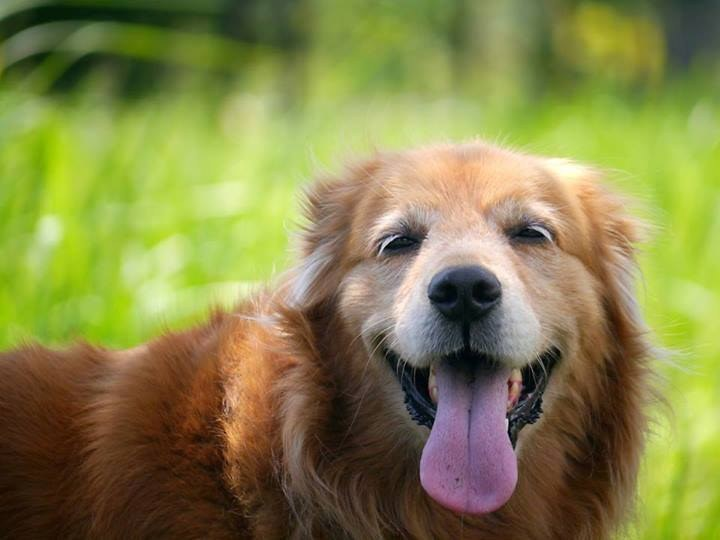
\includegraphics[width=\linewidth]{Figures/dog.jpg}
    \end{minipage}
\end{eg}

Note what the training signal is. It is not the correct label \(y_n\) but a
triple \((\bm{x}, \tilde{y}, \text{goodness})\): some action was taken, and we
learn only how good \emph{that} action was --- never what the best one would
have been. Other problems of the same shape: (customer, ad choice, ad click
earning) \(\Rightarrow\) ad system; (cards, strategy, winning amount)
\(\Rightarrow\) black jack agent.

\begin{moral}
    Reinforcement: learn with `partial/implicit information' (often
    sequentially).
\end{moral}

\subsection{Mini Summary}

\begin{note}[Learning with different data label \(y_n\)]
    \hfill
    \begin{itemize}
        \item supervised: all \(y_n\);
        \item unsupervised: no \(y_n\);
        \item semi-supervised: some \(y_n\);
        \item reinforcement: implicit \(y_n\) by
            \(\text{goodness}(\tilde{y}_n)\);
        \item \ldots{} and more!!
    \end{itemize}
\end{note}

\begin{moral}
    Core tool: supervised learning.
\end{moral}

\begin{exercise}[Fun Time]
    To build a tree recognition system, a company decides to gather one million
    pictures on the Internet. Then it asks each of its \(10\) members to view
    \(100\) pictures and record whether each picture contains a tree. The
    pictures and records are then fed to a learning algorithm to build the
    system. What type of learning problem does the algorithm need to solve?
    \begin{enumerate}[(1)]
        \item supervised;
        \item unsupervised;
        \item semi-supervised;
        \item reinforcement.
    \end{enumerate}
\end{exercise}

\begin{proof}[Reference Answer]
    (3). The \(1{,}000\) records are the labelled \((\bm{x}_n, y_n)\); the other
    \(999{,}000\) pictures are unlabelled \(\bm{x}_n\).
\end{proof}

\section{Learning with Different Protocol
\texorpdfstring{\(f \Rightarrow (\bm{x}_n, y_n)\)}{f => (xn,yn)}}\label{sec:protocol}

\source{slides p.16--21}

The third slot is not about what the data \emph{is} but about how it reaches the
algorithm --- the arrow from \(f\) down to \(\mathcal{D}\).

\subsection{Batch Learning}

\begin{definition}[Batch learning]\label{def:batch}
    Under the \vocab{batch} protocol the entire \(\mathcal{D}\) is handed to
    \(\mathcal{A}\) at once, and \(\mathcal{A}\) returns a single hypothesis
    \(g\) that is then held fixed.
\end{definition}

\begin{eg}
    \begin{enumerate}
        \item The coin recogniser of \autoref{eg:coins} is handed its whole data set at once and learns from all of it: batch supervised multiclass classification.
        \item a batch of (email, spam?) \(\Rightarrow\) spam filter
        \item a batch of (patient, cancer) \(\Rightarrow\) cancer classifier; a batch of patient data \(\Rightarrow\) groups of patients
    \end{enumerate}
\end{eg}
\begin{remark}
    The last one unsupervised, so the protocol is independent of the previous two sections.
\end{remark}

\begin{moral}
    Batch learning: a very common protocol.
\end{moral}

\subsection{Online Learning}

\begin{definition}[Online learning]\label{def:online}
    Under the \vocab{online} protocol the examples arrive one at a time: at step
    \(t\) the learner sees \(\bm{x}_t\), predicts with its current \(g_t\), is
    then told \(y_t\), and updates to \(g_{t+1}\). There is no separate training
    phase --- the hypothesis in use is the one still being learned.
\end{definition}

\begin{eg}[A spam filter that improves]
    A \emph{batch} spam filter learns from known (email, spam?) pairs and then
    predicts with a fixed \(g\). An \emph{online} spam filter instead repeats,
    for \(t = 1, 2, \dots\):
    \begin{enumerate}
        \item observe an email \(\bm{x}_t\);
        \item predict its spam status with the current \(g_t(\bm{x}_t)\);
        \item receive the `desired label' \(y_t\) from the user, and then update
            \(g_t\) with \((\bm{x}_t, y_t)\).
    \end{enumerate}
\end{eg}

\begin{question}
    Two connections to what we have already learned: PLA can be easily adapted
    to the online protocol --- how? And reinforcement learning is often done
    online --- why?
\end{question}

\begin{proof}[Answer]
    PLA already works one example at a time: it looks at a single
    \((\bm{x}_{n(t)}, y_{n(t)})\), and either leaves \(\bm{w}\) alone or
    corrects it. Feed it a stream instead of a fixed \(\mathcal{D}\) and nothing
    in \autoref{alg:pla} has to change. Reinforcement learning is online almost
    by definition: the signal \((\bm{x}, \tilde{y}, \text{goodness})\) only
    exists once an action has been taken, so the data cannot be collected in
    advance --- it is generated by the learner's own behaviour.
\end{proof}

\begin{moral}
    Online: the hypothesis `improves' through receiving data instances
    sequentially.
\end{moral}

\subsection{Active Learning}

\begin{definition}[Active learning]\label{def:active}
    Under the \vocab{active} protocol the learner \emph{chooses} which
    \(\bm{x}_n\) it wants labelled and queries that label, instead of accepting
    whichever examples happen to arrive. The aim is to reach a good \(g\) from
    fewer labels by asking about the inputs that are most informative.
\end{definition}

\begin{center}
    \begin{adjustbox}{max width=\textwidth}
        \begin{tikzpicture}
            \node[mlbox, minimum width=4.2cm] (f) at (0,2.25)
                {unknown target function\\
                 \(f\colon \mathcal{X} \to \mathcal{Y}\)\\[2pt]
                 {\scriptsize (ideal target formula)}};
            \node[mlbox, minimum width=5.2cm] (D) at (0,0)
                {training examples\\
                 \(\mathcal{D}\colon (\bm{x}_1, y_1), \dots , (\bm{x}_N, y_N)\)\\[2pt]
                 {\scriptsize (historical records)}};
            \node[mlop, minimum width=2.4cm] (A) at (5.4,0)
                {learning\\algorithm\\\(\mathcal{A}\)};
            \node[mlbox, minimum width=4.4cm] (g) at (10.2,0)
                {final hypothesis\\\(g \approx f\)\\[2pt]
                 {\scriptsize (`learned' formula to be used)}};
            \node[mlbox, minimum width=3.4cm] (H) at (5.4,-2.25)
                {hypothesis set\\\(\mathcal{H}\)\\[2pt]
                 {\scriptsize (set of candidate formulas)}};
            \draw[mlarrow, draw=WildStrawberry, very thick] (f)
                -- node[right=1pt, font=\scriptsize, WildStrawberry] {protocol} (D);
            \draw[mlarrow] (D) -- (A);
            \draw[mlarrow] (A) -- (g);
            \draw[mlarrow] (H) -- (A);
            \draw[mlarrow, draw=Orange, very thick] (A.north)
                to[out=140, in=-25] (f.east);
        \end{tikzpicture}
    \end{adjustbox}
\end{center}

\begin{note}[Protocol \(\iff\) learning philosophy]
    \hfill
    \begin{itemize}
        \item batch: `duck feeding' --- everything is pushed in at once;
        \item online: `passive sequential' --- take what arrives, in order;
        \item active: `question asking' (sequentially) --- query the \(y_n\) of
            a \emph{chosen} \(\bm{x}_n\).
    \end{itemize}
\end{note}

\begin{moral}
    Active: improve the hypothesis with fewer labels (hopefully) by asking
    questions strategically.
\end{moral}

\subsection{Mini Summary}

\begin{note}[Learning with different protocol \(f \Rightarrow (\bm{x}_n, y_n)\)]
    \hfill
    \begin{itemize}
        \item batch: all known data;
        \item online: sequential (passive) data;
        \item active: strategically-observed data;
        \item \ldots{} and more!!
    \end{itemize}
\end{note}

\begin{moral}
    Core protocol: batch.
\end{moral}

\begin{exercise}[Fun Time]
    A photographer has \(100{,}000\) pictures, each containing one baseball
    player. He wants to categorize the pictures automatically by the player
    inside. He starts by categorizing \(1{,}000\) pictures himself, and then
    writes an algorithm that tries to categorize the other pictures if it is
    `confident' on the category, while pausing for --- and learning from ---
    human input if not. What protocol best describes the nature of the
    algorithm?
    \begin{enumerate}[(1)]
        \item batch;
        \item online;
        \item active;
        \item random.
    \end{enumerate}
\end{exercise}

\begin{proof}[Reference Answer]
    (3). The algorithm takes an active but naïve strategy: ask when `confused'.
    You should probably do the same when taking a class. :-)
\end{proof}

\section{Learning with Different Input Space
\texorpdfstring{\(\mathcal{X}\)}{X}}\label{sec:inspace}

\source{slides p.22--28}

\subsection{Concrete Features}

\begin{definition}[Concrete features]\label{def:concrete}
    \(\mathcal{X} \subseteq \mathbb{R}^d\) consists of \vocab{concrete features}
    when each of its \(d\) dimensions carries a sophisticated physical meaning
    --- annual salary, mass, tumour size --- normally because a human who
    understood the task chose to measure it.
\end{definition}

\begin{center}
    \begin{adjustbox}{max width=\textwidth}
        \begin{tikzpicture}
            \node[mlbox, minimum width=4.2cm] (f) at (0,2.25)
                {unknown target function\\
                 \(f\colon\) \textcolor{WildStrawberry}{\(\bm{\mathcal{X}}\)} \(\to \mathcal{Y}\)\\[2pt]
                 {\scriptsize (ideal target formula)}};
            \node[mlbox, minimum width=5.2cm] (D) at (0,0)
                {training examples\\
                 \(\mathcal{D}\colon (\bm{x}_1, y_1), \dots , (\bm{x}_N, y_N)\)\\[2pt]
                 {\scriptsize (historical records)}};
            \node[mlop, minimum width=2.4cm] (A) at (5.4,0)
                {learning\\algorithm\\\(\mathcal{A}\)};
            \node[mlbox, minimum width=4.4cm] (g) at (10.2,0)
                {final hypothesis\\\(g \approx f\)\\[2pt]
                 {\scriptsize (`learned' formula to be used)}};
            \node[mlbox, minimum width=3.4cm] (H) at (5.4,-2.25)
                {hypothesis set\\\(\mathcal{H}\)\\[2pt]
                 {\scriptsize (set of candidate formulas)}};
            \draw[mlarrow] (f) -- (D);
            \draw[mlarrow] (D) -- (A);
            \draw[mlarrow] (A) -- (g);
            \draw[mlarrow] (H) -- (A);
            \node[mlbox, minimum width=4.8cm] (side) at (8.30,2.55)
                {\scriptsize\textbf{Applicant Information}\\[3pt] \scriptsize\begin{tabular}{@{}lr@{}}age & 23 years\\ gender & female\\ annual salary & NTD 1,000,000\\year in residence & 1 year\\ year in job & 0.5 year\\current debt & 200,000\\\end{tabular}};
        \end{tikzpicture}
    \end{adjustbox}
\end{center}

\begin{moral}
    Concrete features: each dimension of \(\mathcal{X} \subseteq \mathbb{R}^d\)
    represents `sophisticated physical meaning'.
\end{moral}

Every input we have met so far is of this kind: \((\text{size},
\text{mass})\) for coin classification, customer information for credit
approval, patient information for cancer diagnosis. What they share is that
somebody decided which quantities were worth measuring --- the features carry
`human intelligence' about the learning task, put there before learning began.

\begin{moral}
    Concrete features: the `easy' ones for ML.
\end{moral}

\subsection{Raw Features}

\begin{definition}[Raw features]\label{def:raw}
    \(\mathcal{X}\) consists of \vocab{raw features} when each dimension has
    only a simple physical meaning --- the darkness of one pixel, one sample of
    a waveform. Any dimension on its own says almost nothing; the information
    lives in combinations of very many of them.
\end{definition}

\begin{eg}[Digit recognition]
    Features \(\Rightarrow\) meaning of digit: a typical supervised multiclass
    classification problem. But what are the features?
    \begin{center}
        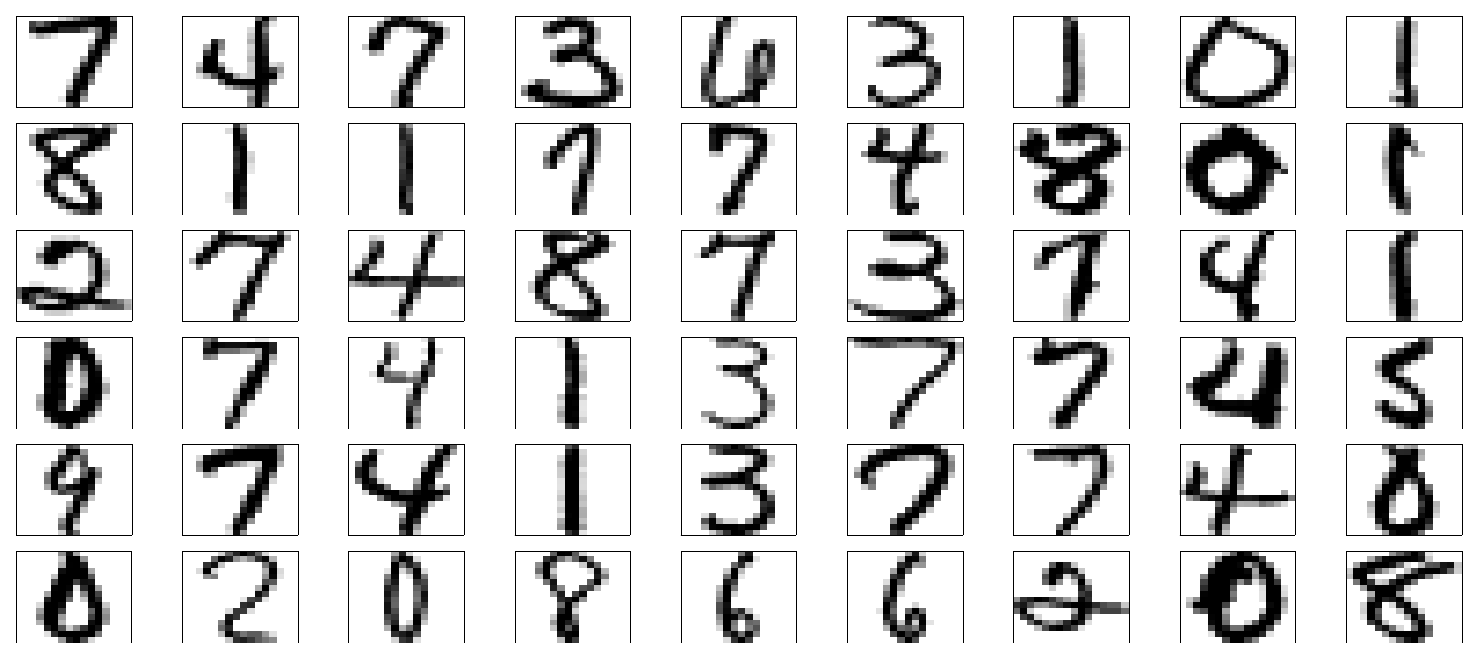
\includegraphics[width=0.78\textwidth]{Figures/digits_raw.png}
    \end{center}
\end{eg}

The honest answer is that a \(16 \times 16\) grey image is just a list of
\(256\) numbers,
\[
    \bm{x} \equiv (0, 0, 0.9, 0.6, \dots) \in \mathbb{R}^{256} ,
\]
and each of those numbers means only `how dark is this one pixel'. That is a
\emph{simple} physical meaning, and it makes the problem harder for machine
learning, not easier --- no single pixel tells you anything about the digit.
Compare what a human would hand over instead: two numbers, symmetry and density,
chosen because they happen to separate the classes.

\begin{center}
    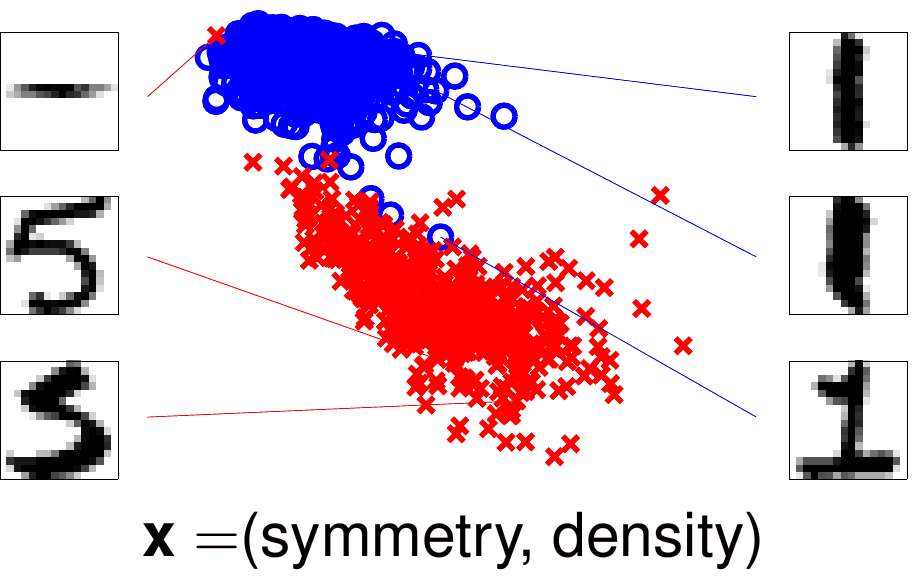
\includegraphics[width=0.62\textwidth]{Figures/digit_features.png}
\end{center}

Other problems with raw features: image pixels, speech signals, and so on.

\begin{moral}
    Raw features: often need humans or machines to convert them to concrete
    ones.
\end{moral}

\subsection{Abstract Features}

\begin{definition}[Abstract features]\label{def:abstract}
    \(\mathcal{X}\) consists of \vocab{abstract features} when its dimensions
    have no (or very little) physical meaning at all --- identifiers such as a
    userid or an itemid, where even the ordering of the numbers is an accident
    of bookkeeping.
\end{definition}

\begin{eg}[Rating prediction, KDDCup 2011]
    Given previous (userid, itemid, rating) tuples, predict the rating that some
    userid would give to some itemid. This is a regression problem with
    \(\mathcal{Y} \subseteq \mathbb{R}\) as the rating and \(\mathcal{X}
    \subseteq \mathbb{N} \times \mathbb{N}\) as (userid, itemid).
\end{eg}

User \(5{,}001\) is not in any sense one more than user \(5{,}000\), so this is
harder still than raw features. Other problems
with abstract features: student IDs in an online tutoring system (KDDCup 2010),
advertisement IDs in an online ad system. That these two competitions were won
by extracting factors from bare IDs is exactly the story of
\autoref{sec:applications}.

\begin{moral}
    Abstract: again needs `feature conversion/extraction/construction'.
\end{moral}

\subsection{Mini Summary}

\begin{note}[Learning with different input space \(\mathcal{X}\)]
    \hfill
    \begin{itemize}
        \item concrete: sophisticated (and related) physical meaning;
        \item raw: simple physical meaning;
        \item abstract: no (or little) physical meaning;
        \item \ldots{} and more!!
    \end{itemize}
\end{note}

\begin{moral}
    `Easy' input: concrete.
\end{moral}

\begin{exercise}[Fun Time]
    Consider the problem of building an online image advertisement system that
    shows users the most relevant images. What features can you choose to use?
    \begin{enumerate}[(1)]
        \item concrete;
        \item concrete, raw;
        \item concrete, abstract;
        \item concrete, raw, abstract.
    \end{enumerate}
\end{exercise}

\begin{proof}[Reference Answer]
    (4). Concrete user features, raw image features, and maybe abstract
    user\slash image IDs.
\end{proof}

\hrulebar

\subsection*{Summary}

\begin{description}
    \item[Output space \(\mathcal{Y}\)] \emph{classification},
        \emph{regression}, structured.
    \item[Data label \(y_n\)] \emph{supervised}, un/semi-supervised,
        reinforcement.
    \item[Protocol \(f \Rightarrow (\bm{x}_n, y_n)\)] \emph{batch}, online,
        active.
    \item[Input space \(\mathcal{X}\)] \emph{concrete}, raw, abstract.
\end{description}

The emphasised entry in each line is the one this course treats as its core
tool, and the combination of all four --- batch supervised binary
classification on concrete features --- is exactly the setting PLA already
solves. Everything else in the list is reached by relaxing one slot at a time.

Which makes the next question awkward. We have a solved case and a map of its
neighbours, but not one word yet about whether any of it works on data we have
never seen. The next chapter argues, seriously, that learning is impossible.
